\section{Verwandte Arbeiten}

\begin{figure*}
    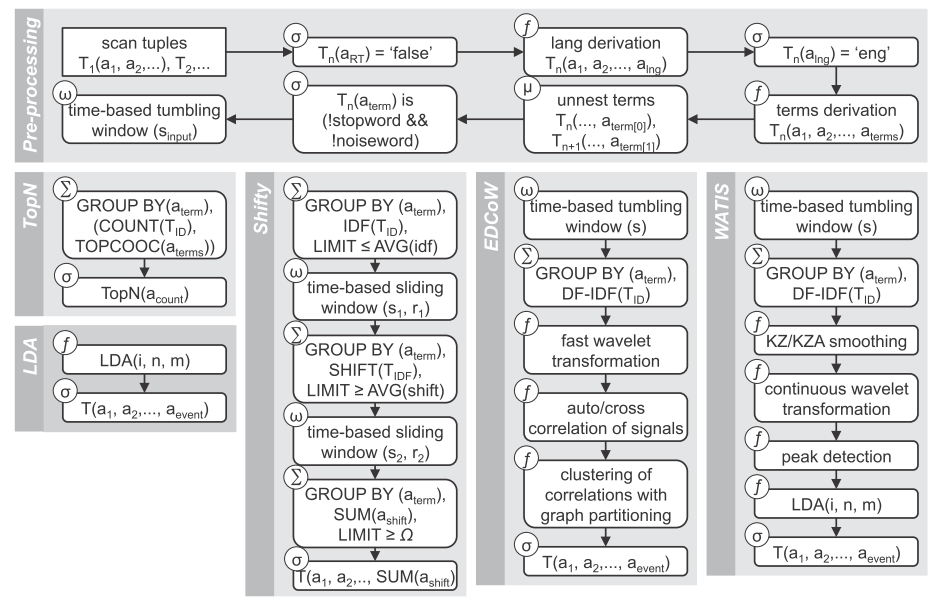
\includegraphics[width=\textwidth]{images/eventdetect.png}
    \caption{Niagarino Anfragen der fünf Erkennungs-Methoden}
    \label{fig:eventdetect}
\end{figure*}

\subsection{Event-Driven Detection}
Weiler et. al. \cite{weiler2016evaluation} evaluieren fünf State of the Art Techniken zur Erkennung von noch unbekannten Ereignissen in einem Event Stream. Als Implementation wird Niagarino verwendet, eine von Weiler et. al. entwickelte Plattform die Apache Storm ähnelt. Die Techniken wurden als Anfragen umgesetzt, wie in Abbildung \ref{fig:eventdetect} dargestellt. Twitter-Events dienen als Datenbasis, die in einem Pre-Processing gefiltert werden. Dabei werden Retweets entfernt und der Inhalt der restlichen Tweets gesäubert, es verbleiben bibliographisch erkannte englische Wörter. 

\begin{itemize}
\item TopN\\Jedem Wort wird ein Wert zugewiesen, der auf dem Inverse-Document-Frequency des Zeitfenster beruht. Häufig vorkommende Wörter die im Allgemeinen selten verwendet werden erhalten die besere Bewertung. Nur die N-wichtigtsten Wörter verbleiben als Event.
\item Latent Dirichlet Allocation (LDA)\\Ist ein hierarchisches Bayes-Modell, das die Variation des Vokabulars in einer Gruppe von Dokumenten bewertet. Für jedes Zeitfenster extrahiert LDA  vermutete Ereignisse, die durch Ausdrücke beschrieben werden. 
\item Shifty\\Dabei werden die Veränderungen von TopN bewertet die sich zwischen zwei Zeitfenstern ereignen.
\item Event Detection with Clustering of
Wavelet-based Signals (EDCoW)\\Der Stream wird in Batches aufgeteilt, die dann per Wavelet-Analyse zu einem weiteren Event zusammengefasst werden. Dieses beinhaltet die Terme die im Zusammenhang mit dem erkannten Burst stehen, wovon unwichtige Wörter entfernt wurden. Durch Clustering enthält das Ergebnis Burst-Events die mit zwei Termen beschreiben werden.
\item Wavelet Analysis Topic Inference Summarization
(WATIS)\\ Eine Weiterentwicklung des (EDCoW), wobei nun zu jedem Burst fünf Terme geliefert werden.
\end{itemize}

\subsection{Burst Detection}
Da sich die Erkennung globaler Events mittels Esper als zumindest unvollständig erwies, wurden Methoden untersucht die das Verfahren  Ergänzen oder Ersetzen können.\\

Globale Events haben unter anderem auch die Eigenschaft eine erhöhte Aktivität im Edit-Event-Stream zu verursachen. Erhöhte Aktivität (Bursts) ist ein Phänomen das bereits seit Jahrzehnten untersucht wird, daher existieren eine Reihe von Theorien und abgeleiteten Algorithmen. Die zeitnahe Erstellung von Ergebnissen ist wichtig, weswegen auf eine schnelle Verarbeitung hin optimiert wird. Bursts besitzen eine Reihe an Attributen, die abhänig vom Use Case defininert werden. Dazu zählt der Zeitraum der jeweils auf das Auftreten eines Bursts untersucht wird, die Intensistät und die Verteilung der Intensistät auf den betrachteten Zeitraum.\\

Generell kann ein Datenstrom auf zwei Methoden betrachtet werden. Beim Point Monitoring wird nur das aktuelle Ereignis betrachtet. Liegt der Wert eines Attributs des Events in einen vordefinierten Bereich oder überschreitet es einen Grenzwert, wird ein Burst erkannt. Beim Aggregate Monitoring werden über einen Zeitraum (Windows) hinweg Ereignisse aggregiert. Drei Zeitfenstertypen werden unterschieden. Beim Landmark Window wird der Zeitraum durch einmalig fest gelegte Zeitpunkte definiert.
Das Sliding Window hingegen bewegt sich durch die Zeit, mit festgelegter Größe und festgelegtem Intervall. Die Parameter können als Zeitangaben oder als Zählangaben erfolgen. Ein Window wird entweder nach einer gewissen Zeit neu erstellt oder nach einer bestimmten Anzahl an Ereignissen. Beim Damped Window werden zudem jedem Ereignis Gewichtungen erteilt, je länger ein Ereignis zurückliegt, desto weniger Gewicht bekommt es mit Fortschreiten der Zeit. \cite{Zhu:2003:EEB:956750.956789}\\

\begin{figure*}[htbp]
\centerline{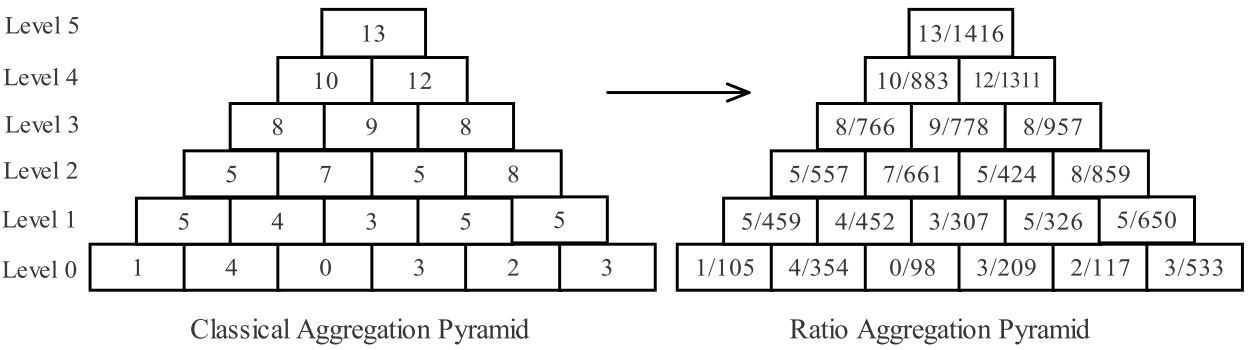
\includegraphics[height=4.4cm]{images/ratiopyramid.png}}
\caption{Von der klassischen 'Aggregataion Pyramid' zur 'Ratio Aggreation Pyramid' \cite{yuan2007online}}
\label{fig:ratiopyramid}
\end{figure*}


\begin{figure}[h]
    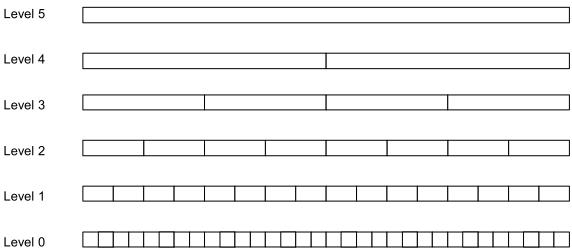
\includegraphics[width=.5\textwidth]{images/wavelet.jpg}
    \caption{Wavelet Tree \cite{Zhu:2003:EEB:956750.956789}}
    \label{fig:wavelet}
\end{figure}

Eine spezielles Modell entwickeln Zhu et. al. in 'Efficient Elastic Burst Detection in Data Streams' \cite{Zhu:2003:EEB:956750.956789} mit dem Elastic Window, bei dem   die Größe der Zeitfenster variiert. Somit können die Bursts dynamischer durch deren Charakteristik und unabhängiger von ihrer Dauer erkannt werden, die oftmals nicht im Vorfeld festgelegt werden kann. Dafür wird ein Wavelet-Tree vom Stream erzeugt, bei dem die Wavelet-Kooefizienten den Aggregaten der Fenster entsprechen. Wie in Abbildung \ref{wavelet} zu sehen ist, wird zu Beginn der Stream in Fenster unterteilt, die disjunkt nebeneinander liegen. Je Fenster wird ein Aggregat erstellt - in der Regel werden dazu die Ereignisse eines bestimmten Typs oder Ereignisse mit gleichen Attributen gezählt. Diese Aggregate bilden nun selbst einen Stream. Das Verfahren wird wiederholt, vorausgesetzt es befinden sich entsprechende Ereignisse bzw. aggregierte Ereignisse im Stream. Mit jedem Schritt wird der betrachtete Zeitabschnitt größer und man bewegt in das nächst höhere Level Richtung Wurzel des Baums. Zu jedem Level wird ein Schwellwert angegeben, bei dessen Überscheitung ein Burst ausgelöst wird.

\begin{figure*}[htbp]
\centerline{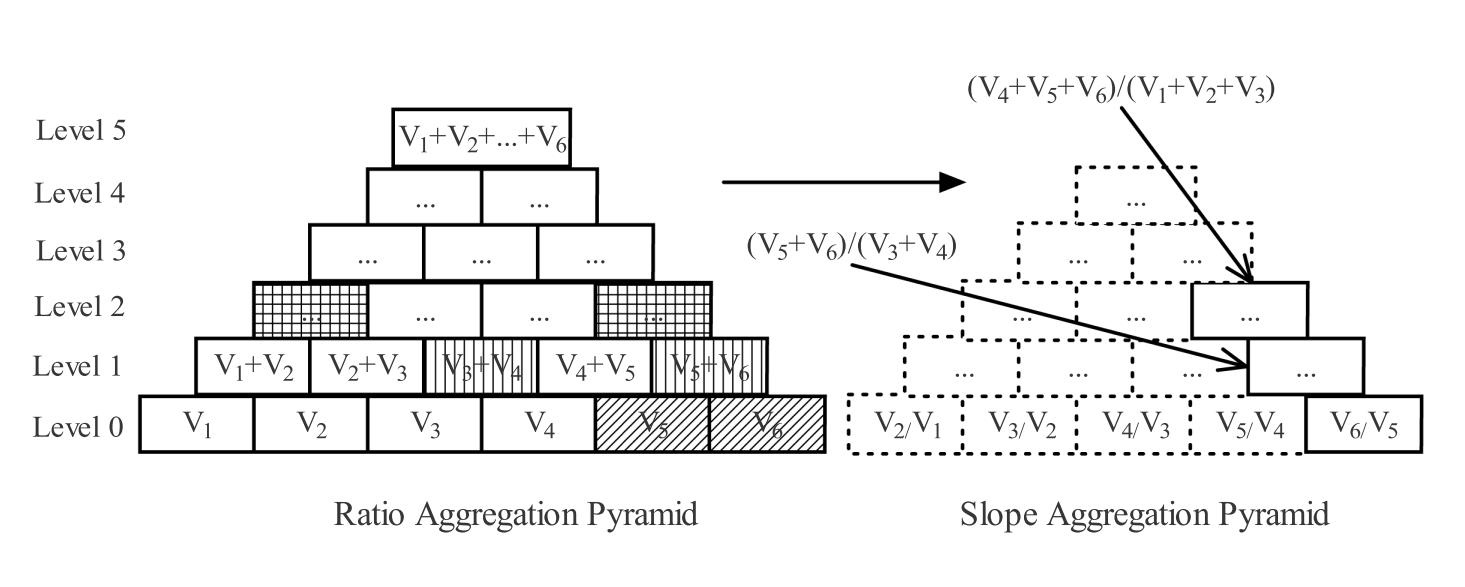
\includegraphics[height=6.3cm]{images/slopepyramid.jpg}}
\caption{Berechnungsbeispiel zur 'Slope Pyramid' \cite{yuan2007online}}
\label{fig:slopepyramid}
\end{figure*}

% \begin{figure*}
%     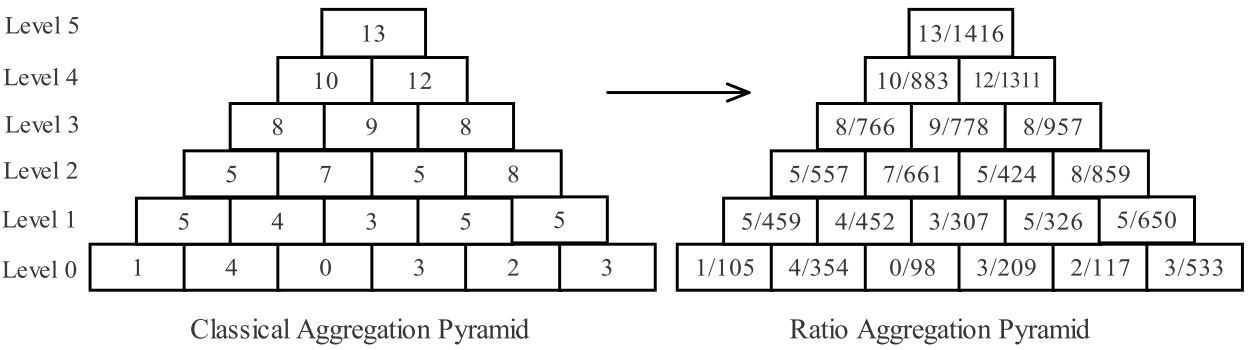
\includegraphics[width.5=\textwidth]{images/ratiopyramid.jpg}
%     \caption{Von der klassischen 'Aggregataion Pyramid' zur 'Ratio Aggreation Pyramid' \cite{yuan2007online}}
%     \label{fig:ratiopyramid}
% \end{figure*}



Yuan et. al. entwickeln in 'Online Burst Detection Over High Speed Short Text Streams' \cite{yuan2007online} ein Verfahren das auf einem Wavelet-Tree basiert. Dieser kann auch als Pyarmide betrachtet werden, mit den Levels die dem Aggregierungsgrad entsprechen. Da die Burst-Detection sich auf den Schwellwert des jeweiligen Lebels stützt, muss dieser zu beginnder Analyse feststehen. Das kann eine Herausforderung sein, denn  die Menge an Ereignissen im Stream muss vor Beginn der Analyse eingeschätzt werden. Um dieses Problem zu lösen werden keine absoluten Angaben der Aggregatwerte verwendet, wie zum Beispiel deren Anzahl. Stattdessen wird angegeben, wieviele relevante Events aggregiert wurden im Verhältnis zu allen aufgetretenen Events im betroffenen Zeitraum. Abbildung \ref{fig:ratiopyramid}. Eine weitere Komprimierung wird durch die Slope Pyramid, wie in Abbildung \ref{fig:slopepyramid} dargestellt, erreicht. Dabei wird der Fokus auf die Veränderung von Fenster zu Fenster gelegt. Dazu wird der Verhältniswert aus der Ratio Pyamid herangezogen; der Wert des aktuellen Fensters wird durch den des vorhergehenden Fenster dividiert.\cite{yuan2007online}\\

Besondere Anforderungen stellt die Realtime-Burst Detection in Verbindung mit der gleichzeitigen Betrachtung mehrerer Fenstergrößen. Übliche Burst-Detektionsverfahren sind für eine Echtzeiterkennung nicht schnell genug, daher wurde von Ebina et. al. \cite{ebina2011real} Burst-Erkennungsmethode weiter entwickelt. Das Ziel ist dabei die Berechnungszeit zu reduzieren, indem redundante Datenaktualisierungen wie bei Yuan et. al. vermieden werden. Dazu werden die Zellen der Slope Pyramid auf effizientere Weise berechnet.\cite{ebina2011real}\\

Je nach Use Case sind auch aufwändigere Analysen wie in 'Event Detection with Burst Information Networks' \cite{ge2016event} notwendig.

% Detecting ‘bursts’ in time series data with Kleinberg’s burst detection algorithm
% \cite{kleinberg1}

\subsection{Social Media Analyse}
Eine ganze Reihe von Arbeiten beschäftigt sich mit der Analyse der Aktivitäten der Wikipedia-Nutzer.

\begin{itemize}
\item Extracting Event-Related Information from Article Updates in Wikipedia \cite{10.1007978-3-642-36973-5_22}
\item Ongoing events in Wikipedia: a cross-lingual case study \cite{gottschalk2017ongoing}
\item How much is Wikipedia Lagging Behind News? \cite{fetahu2015much}
\item Event analysis in social multimedia: a survey \cite{liu2016event}
\item A cloud-enabled automatic disaster analysis system of multi-sourced data streams: An example synthesizing social media, remote sensing and Wikipedia data \cite{huang2017cloud}
\end{itemize}

% Des weiteren 

% Pinterest
% I need to try this?: a statistical overview of pinterest
% \cite{gilbert2013need}

% Twitter
% An evaluation of the run-time and task-based performance of event detection techniques for Twitter
% \cite{weiler2016evaluation}
